\documentclass[a4paper]{article}

\usepackage[spanish, es-tabla, es-nodecimaldot]{babel}
\usepackage[T1]{fontenc}
\usepackage[utf8]{inputenc}
\usepackage{lmodern}
\usepackage{amsmath, amssymb}
\usepackage{stackengine}
\usepackage{graphicx}
\usepackage[hmargin=1.8cm, vmargin=2cm]{geometry}
\usepackage[separate-uncertainty=true, per-mode=symbol]{siunitx}
\usepackage[small]{titlesec}
\usepackage[bottom]{footmisc}
\usepackage{float}
\usepackage{enumitem}
\usepackage{tikz}
\usepackage[font=small, labelfont=bf, labelsep=period]{caption}
\usepackage{subcaption}
\usepackage[colorlinks=true]{hyperref}

\newcommand{\letrita}[1]{\textsf{\textbf{\footnotesize{(#1)}}}} 

\title{\large{\textbf{Caracterización del generador de número aleatorios del Kilobot o \emph{Moneda}}}}
\author{%
	\normalsize{Tomás Ayala y Romina D'Alessandro}
}
\date{}

\begin{document}
	
\maketitle

Corrimos \href{https://github.com/rldromina/Kilobots/blob/tom/Moneda/moneda.c}{\texttt{moneda.c}}, usando siempre la función \texttt{rand\_hard()}.
Dejamos fijo el tiempo mínimo de prendido/apagado del LED del Kilobot a \texttt{TIME = 1000} (milisegundos).
Registramos varias filmaciones de 15 minutos del Kilobot ``tirando la moneda'' y una de 1 hora.

De cada medición obtenemos un \texttt{.csv} que en sus columnas tiene (i) la intensidad (en un entorno) del LED, con valores entre 0 y 255, y (ii) el instante del tiempo correspondiente. Graficamos la evolución temporal $I(t)$, su autocorrelación (ver la función \texttt{autocorrelacion} de \href{https://github.com/rldromina/Kilobots/blob/tom/Moneda/aux.py}{\texttt{aux.py}}) y la frecuencia con las que ocurren las consecutividades\footnote{¿Existe esta palabra?} de longitud $n$. Por ejemplo, si la moneda en una tirada arrojó HTHTTTHHTHHHHHH, la consecutividad de longitud $n=1$ se presentó $4$ veces (H,T,H,T); la de $n=2$, $1$ vez (HH); la de $n=3$, 1 vez (TTT); la de $n=4$ y $n=5$, ninguna y $n=6$, 1 vez (HHHHHH). Notar que consecutividades de cara o ceca contribuyen por igual.

\begin{figure}[!h]
	\centering
	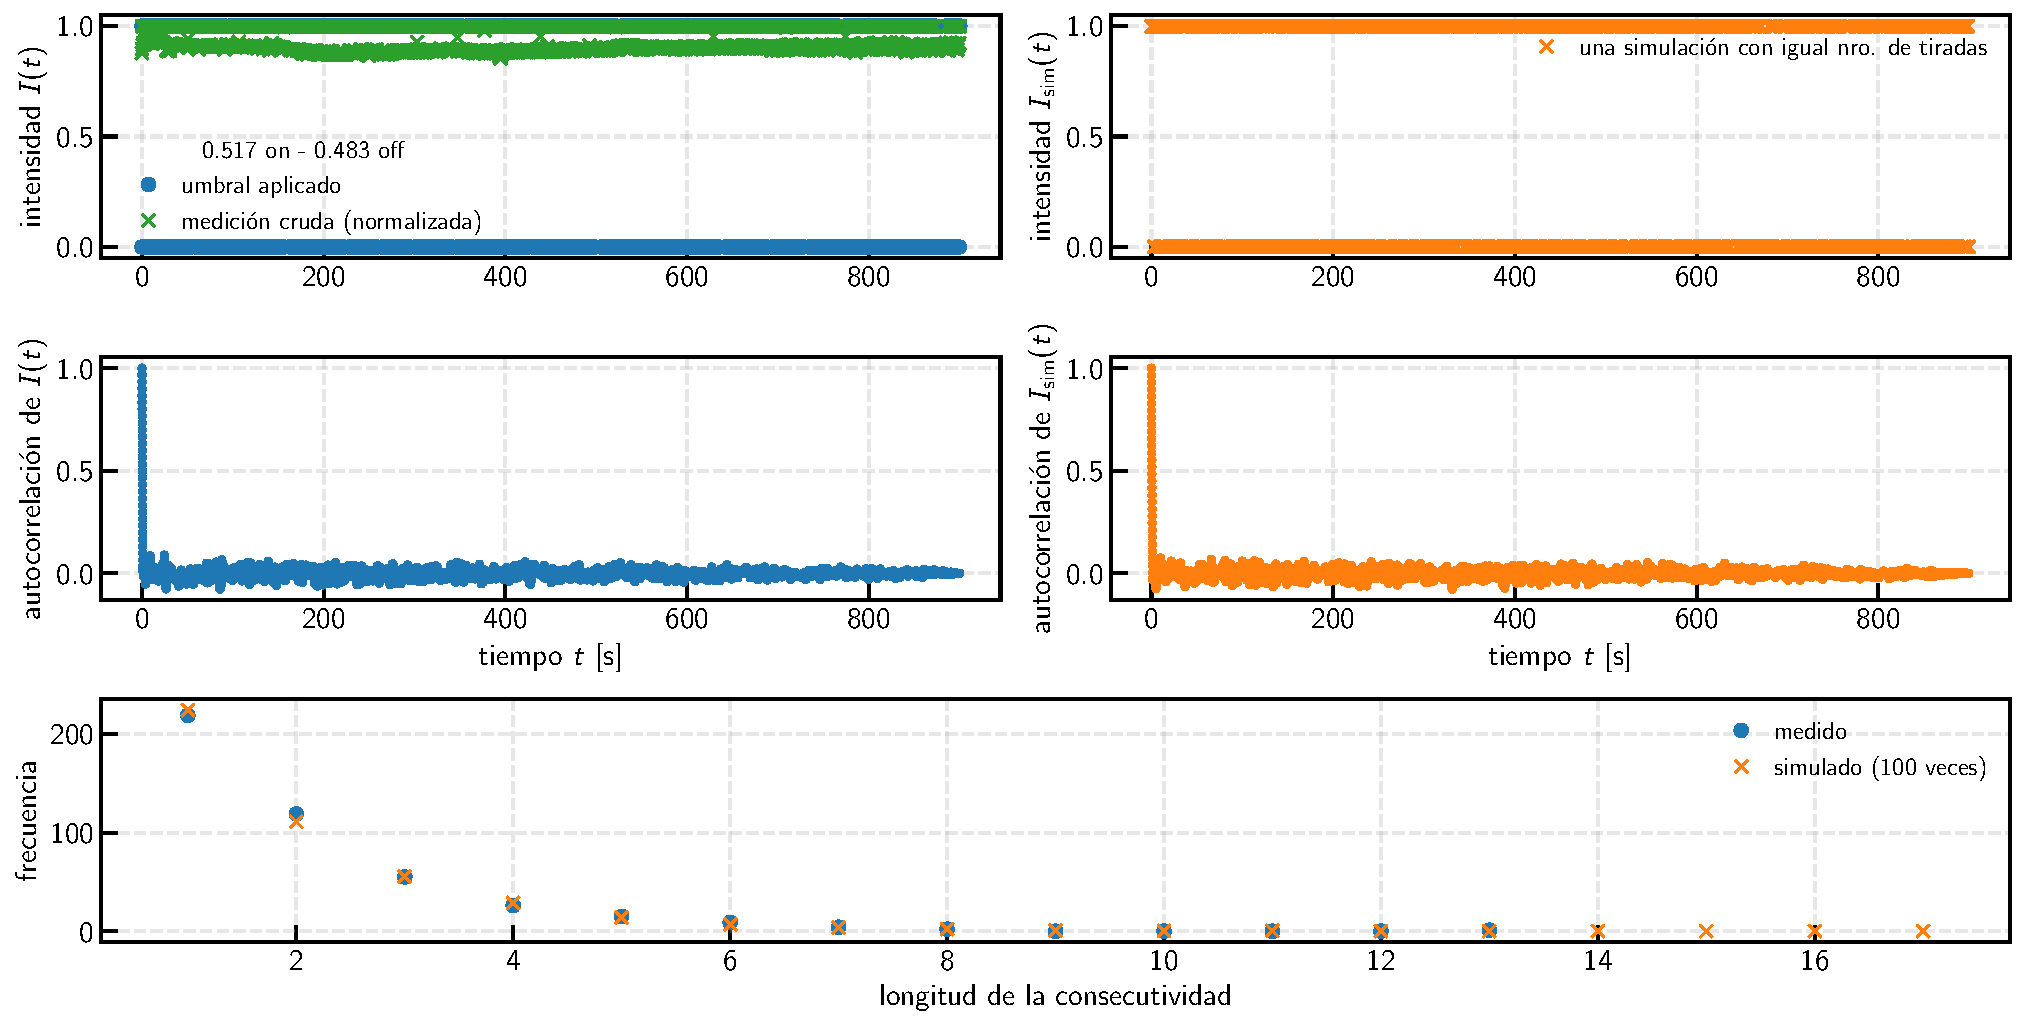
\includegraphics[width=\linewidth]{Resultados/15min_b.pdf}
	\caption{15 minutos.}
\end{figure}

\end{document}